\problemname{Ríkjafræði 1}
\illustration{0.3}{snake}{Mynd fengin af \href{https://commons.wikimedia.org/wiki/File:Snake_lemma_complete.svg}{commons.wikimedia.org}}

Jörmunrekur varði páskafríinu sínu í að kynna sér stærðfræðigrein sem kallast ríkjafræði. Hún notast mikið við
örvarit til að setja fram hugmyndir með myndrænum hætti. Þessar myndir tákna ríki sem samanstanda af hlutum og örvum
milli hluta. Mikilvægur eiginleiki flestra slíkra örvarita er að þau séu víxlin. Það þýðir að ef lagt er af stað frá
einum hlut $A$ og farið er eftir einhverri runu örva að hlut $B$ þá á útkoman úr því ávallt að vera sú sama, óháð hvaða
leið er farin. Jörmunrekur er hér að skoða tiltekið örvarit og er að velta fyrir sér hvort það sé raunverulega víxlið.
Í þessu örvariti er hver hlutur hið venjulega þrívíða rúm og hver ör er hliðrun rúmsins. Örvarnar
eru því gefnar á forminu $(x, y, z)$ sem merkir að punktum er hliðrað um $x$ í $x$-stefnu, $y$ í $y$-stefnu og $z$ í $z$-stefnu.

\section*{Inntak}
Inntak byrjar á einni línu með tveimur heiltölum $1 \leq n \leq 10^5$ og $1 \leq m \leq 10^5$ þar sem $n$ er fjöldi hluta og
$m$ er fjöldi örva. Hlutirnir eru númeraðir frá $1$ og upp í $n$. Næst fylgja $m$ línur, hver með $5$ heiltölum
$1 \leq a, b \leq n$, $-10^9 \leq x, y, z \leq 10^9$. Þetta gefur að í örvaritinu sé ör frá $a$ til $b$ sem
táknar hliðrunina um $(x, y, z)$. Athugið að þar sem örin er gagntæk er sjálfkrafa einnig ör frá $b$ til $a$ sem hliðrar
rúminu um $(-x, -y, -z)$.

\section*{Úttak}
Skrifið út \texttt{Jebb} ef ritið er víxlið, annars \texttt{Neibb}.

\section*{Stigagjöf}
\begin{tabular}{|l|l|l|}
\hline
Hópur & Stig & Takmarkanir \\ \hline
1 & 50 & $1 \leq n \leq 200$ \\ \hline
2 & 50 & Engar frekari takmarkanir \\ \hline
\end{tabular}

\section*{Útskýring á sýnidæmum}
Í fyrra sýnidæminu eru tvær leiðir frá $1$ til $4$. Sama hvor leið er tekin fæst hliðrun $(1,1,1)$ svo þetta rit er víxlið. \\

\begin{figure}[h!]
  \centering
    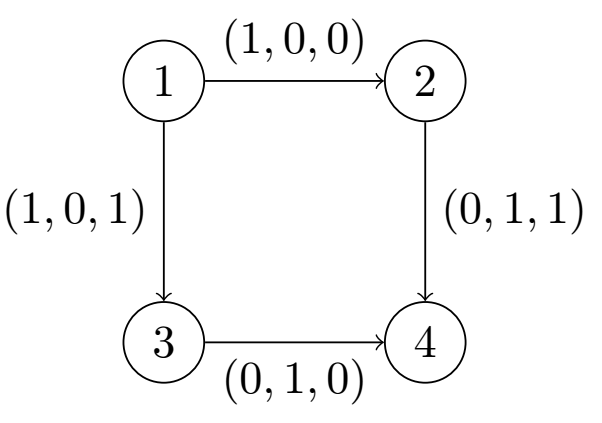
\includegraphics[width=0.5\textwidth]{sample1}
  \caption{Sýnidæmi 1}
\end{figure}

Í seinna sýnidæminu er búið að bæta við öðrum legg. Ef við ferðumst eftir honum afturábak frá $1$ til $4$ er hliðrunin $(-1,-1,-1)$ sem er ekki það sama og hinar leiðirnar. Því er þetta rit ekki víxlið. \\

\begin{figure}[h!]
  \centering
    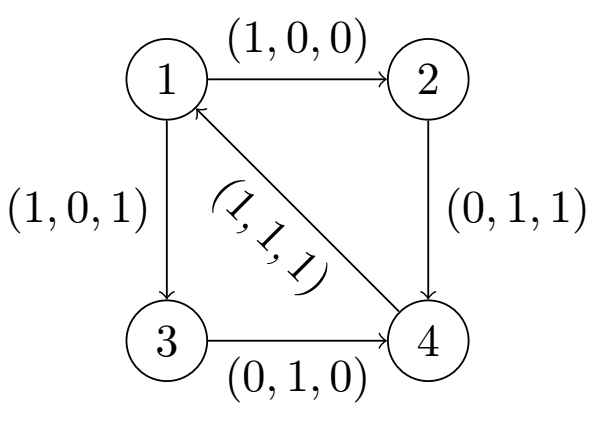
\includegraphics[width=0.5\textwidth]{sample2}
  \caption{Sýnidæmi 2}
\end{figure}
